\documentclass{report}

\usepackage{float}
\usepackage{titlesec}
\usepackage{graphicx}
\usepackage{amsmath}
\usepackage{subcaption}
\usepackage{listings}
\usepackage{xcolor}
\usepackage{apacite}

\bibliographystyle{apacite}

\graphicspath{ {./assets/} {..} }

\newcommand{\subimgw}{.5\linewidth}

\definecolor{codegreen}{rgb}{0,0.6,0}
\definecolor{codegray}{rgb}{0.5,0.5,0.5}
\definecolor{codepurple}{rgb}{0.58,0,0.82}
\definecolor{backcolour}{rgb}{0.95,0.95,0.92}

\lstdefinestyle{mys}{
    backgroundcolor=\color{backcolour},   
    commentstyle=\color{codegreen},
    keywordstyle=\color{magenta},
    numberstyle=\tiny\color{codegray},
    stringstyle=\color{codepurple},
    basicstyle=\ttfamily\footnotesize,
    breakatwhitespace=false,
    breaklines=true,
    captionpos=b,
    keepspaces=true,
    numbers=left,
    numbersep=5px,
    showspaces=false,
    showstringspaces=false,
    showtabs=false,
    tabsize=2
}
\lstset{style=mys}

\author{
  Kristian Henrik Salen Sørli
  \and
  William B. Sørensen\\
}
\title{TOF Rapport}
\begin{document}
\maketitle

\tableofcontents

\chapter{Oppgaver}

% Oppgave 1: Utforske styrken til geometriske strukturer

% 1A: Lag formene nedenfor ved å bruke spagetti og limpistol. Undersøk og sammenlign strukturene sin evne til å bære en vertikal last. Undersøk og sammenlign også hvordan formene reagerer på horisontal last.

% I besvarelsen må dere ta med figurenes korrekte navn, skisse av strukturene og spagetti-strukturene, resultatene fra testingen, teori som kan forklare resultatene dere får fra testingen og endelig konklusjon.

% 1B: Lag formene nedenfor ved å bruke spagetti og limpistol. Undersøk og sammenlign strukturene sin evne til å bære en vertikal last. Undersøk og sammenlign også hvordan formene reagerer på horisontal last.

% I besvarelsen må dere ta med figurenes korrekte navn, skisse av strukturene og spagetti-strukturene, resultatene fra testingen, teori som kan forklare resultatene dere får fra testingen og endelig konklusjon.

\section{Oppgave 1}

\subsection{A}

I denne oppgaven ble det laget en rekke figurer ut av spagettis. Grunnen til dette var for å se hvordan effekt forskyvings kreftene hadde på de forskjellige figurene med å se hvilken av sidene knakk når figuren ble underlagt trykk.

Fra et polygonalt perspektiv er den mest uniformt integral figuren en likesidet trekant. Dette kommer av at den tåler like mye trekk og forskyvning krefter fra hver side av figuren gjennom at den fordeler krafta likt.

En likebeint trekant er sterkest på den korteste siden. Grunnen til dette er siden forskyvnings-kraften blir fordelt over de to lengere sidene.

En rettvinklet trekant er sterkest på den korteste katen.

En firkant er svakest siden den har mulighet til å oppleve plan-forskyvning.

\subsection{B}

Triangulær pyramide har de samme styrkene som en likesidet trekant hvor hvor den tåler fra hver av sidene og den fordeler likt gjennom hele figuren

\begin{figure}[H]
	\begin{subfigure}{.5\textwidth}
		\centering
		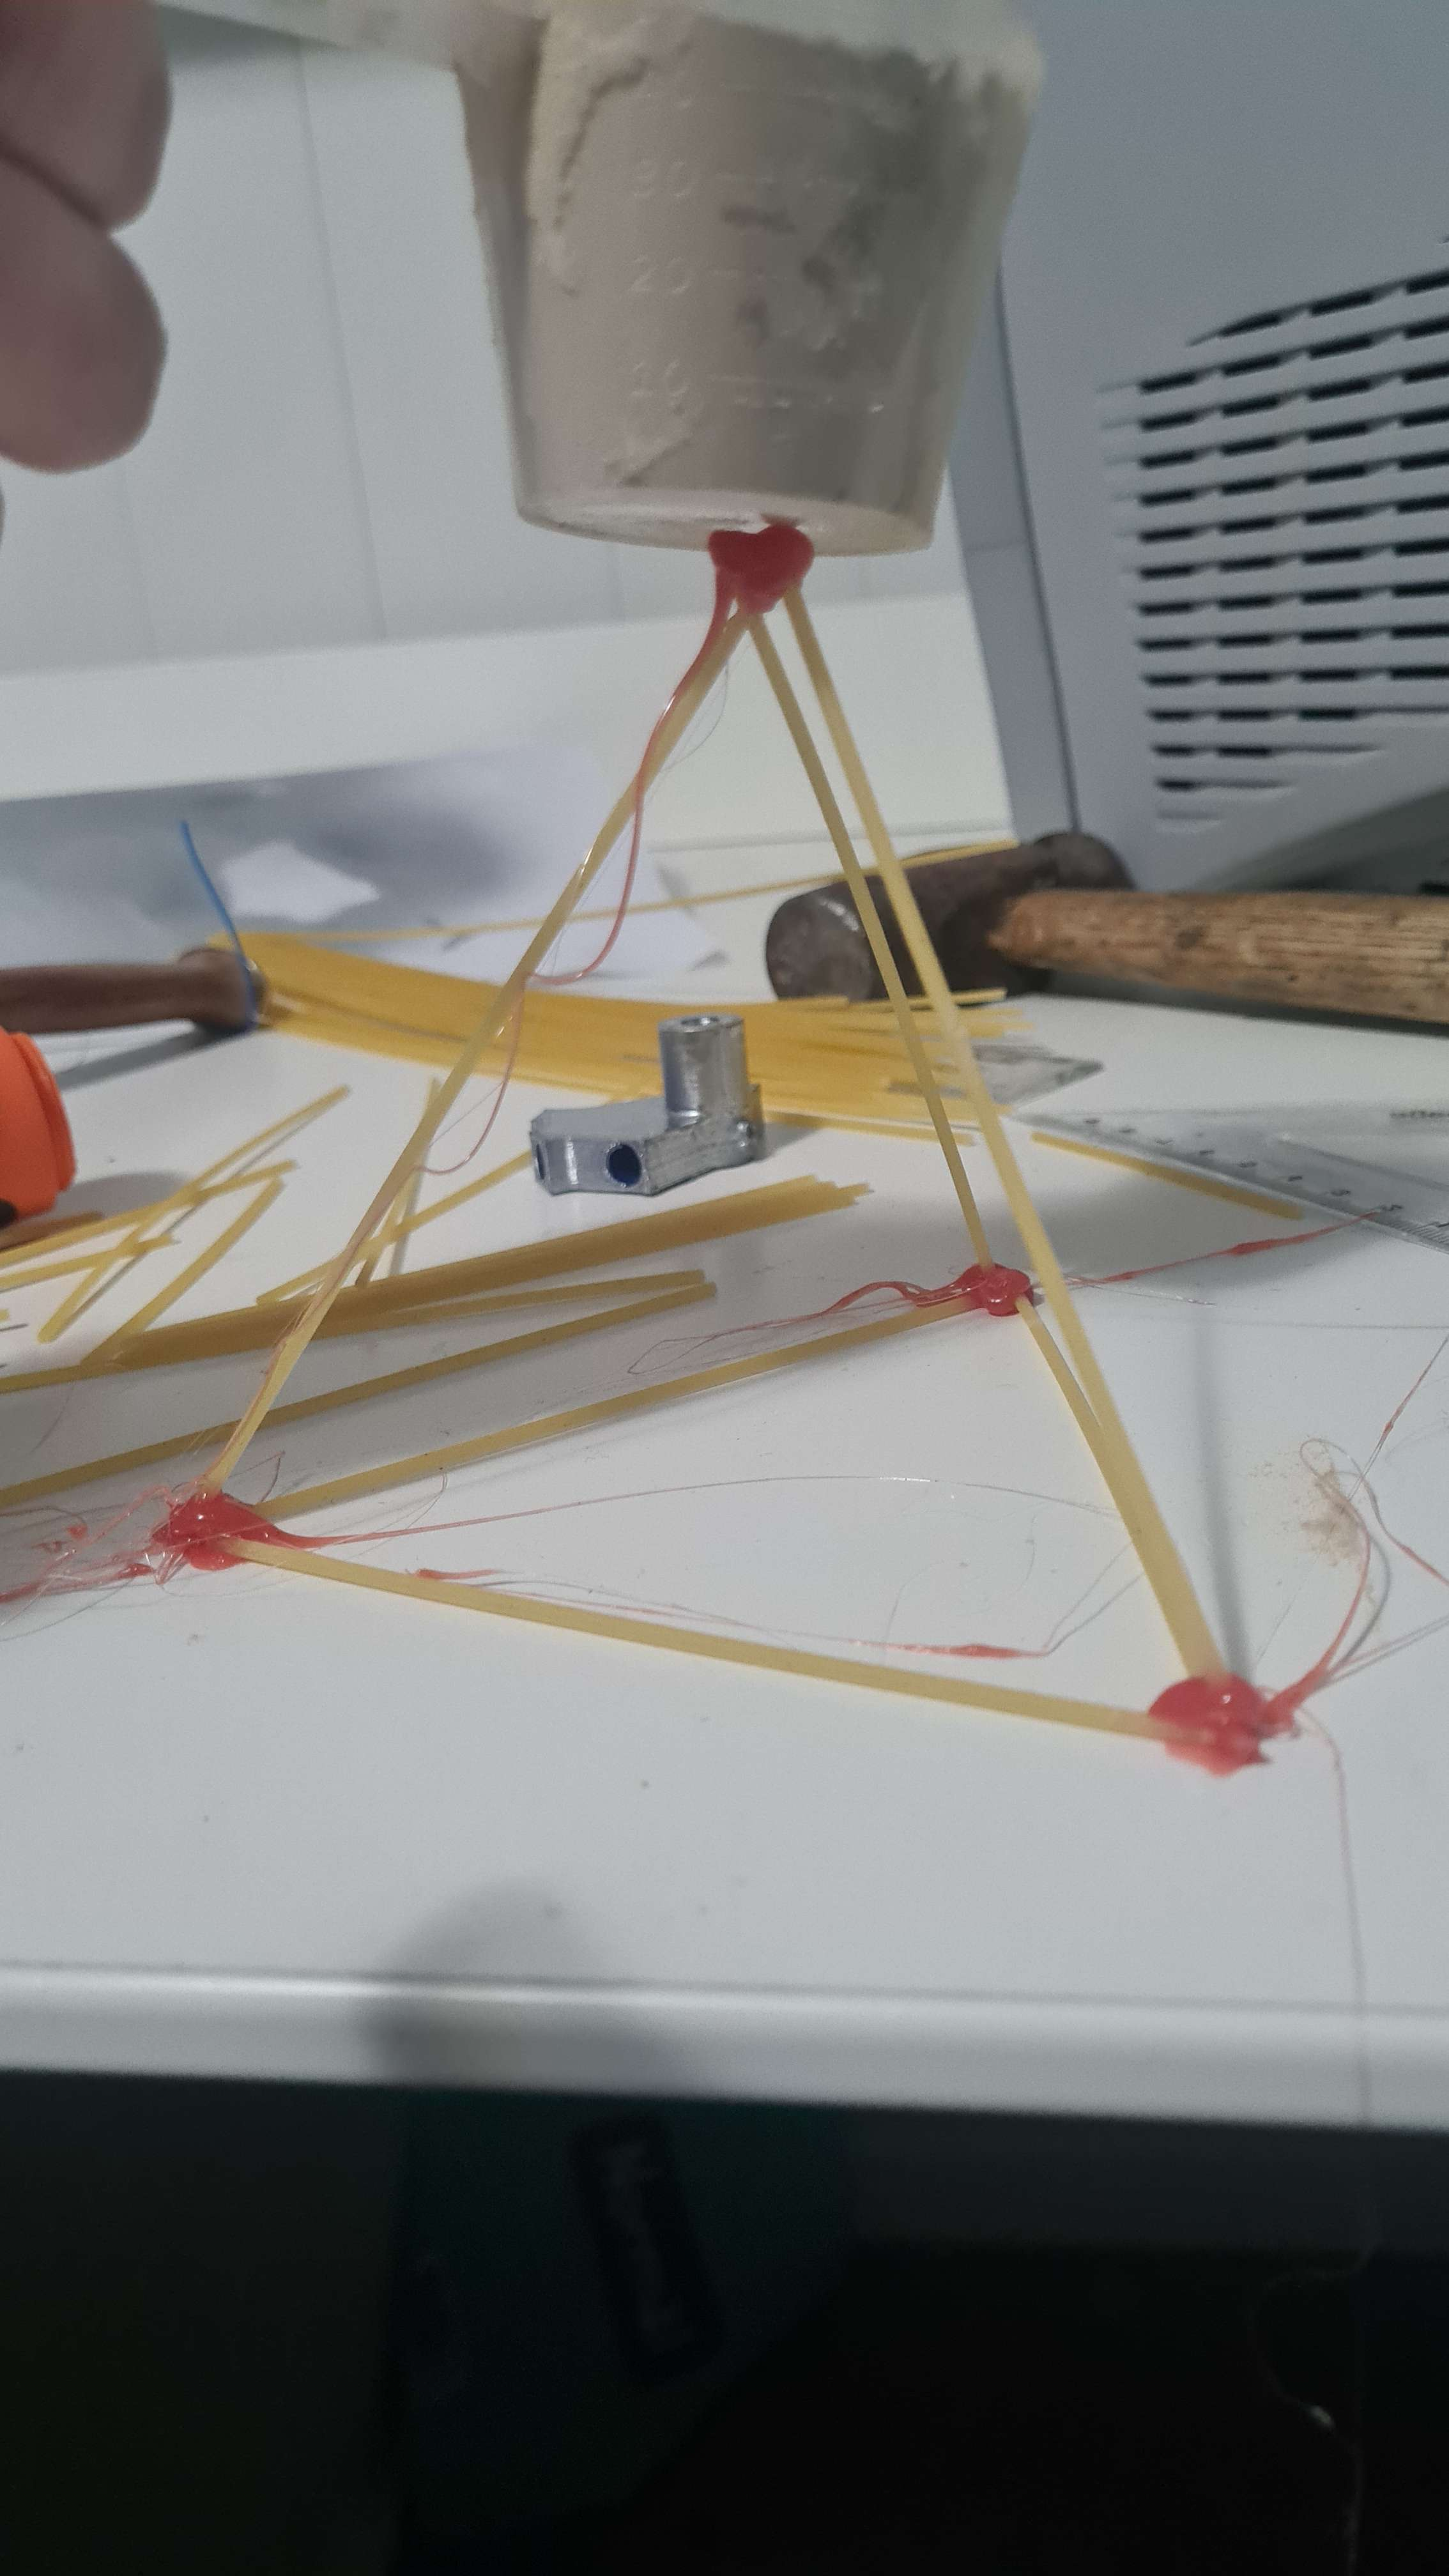
\includegraphics[width=\subimgw]{tetrehedra-a}
		\caption{Compression bucle isomorphism}

		\label{fig:tetrehedra:a}
	\end{subfigure}%
	\begin{subfigure}{.5\textwidth}
		\centering
		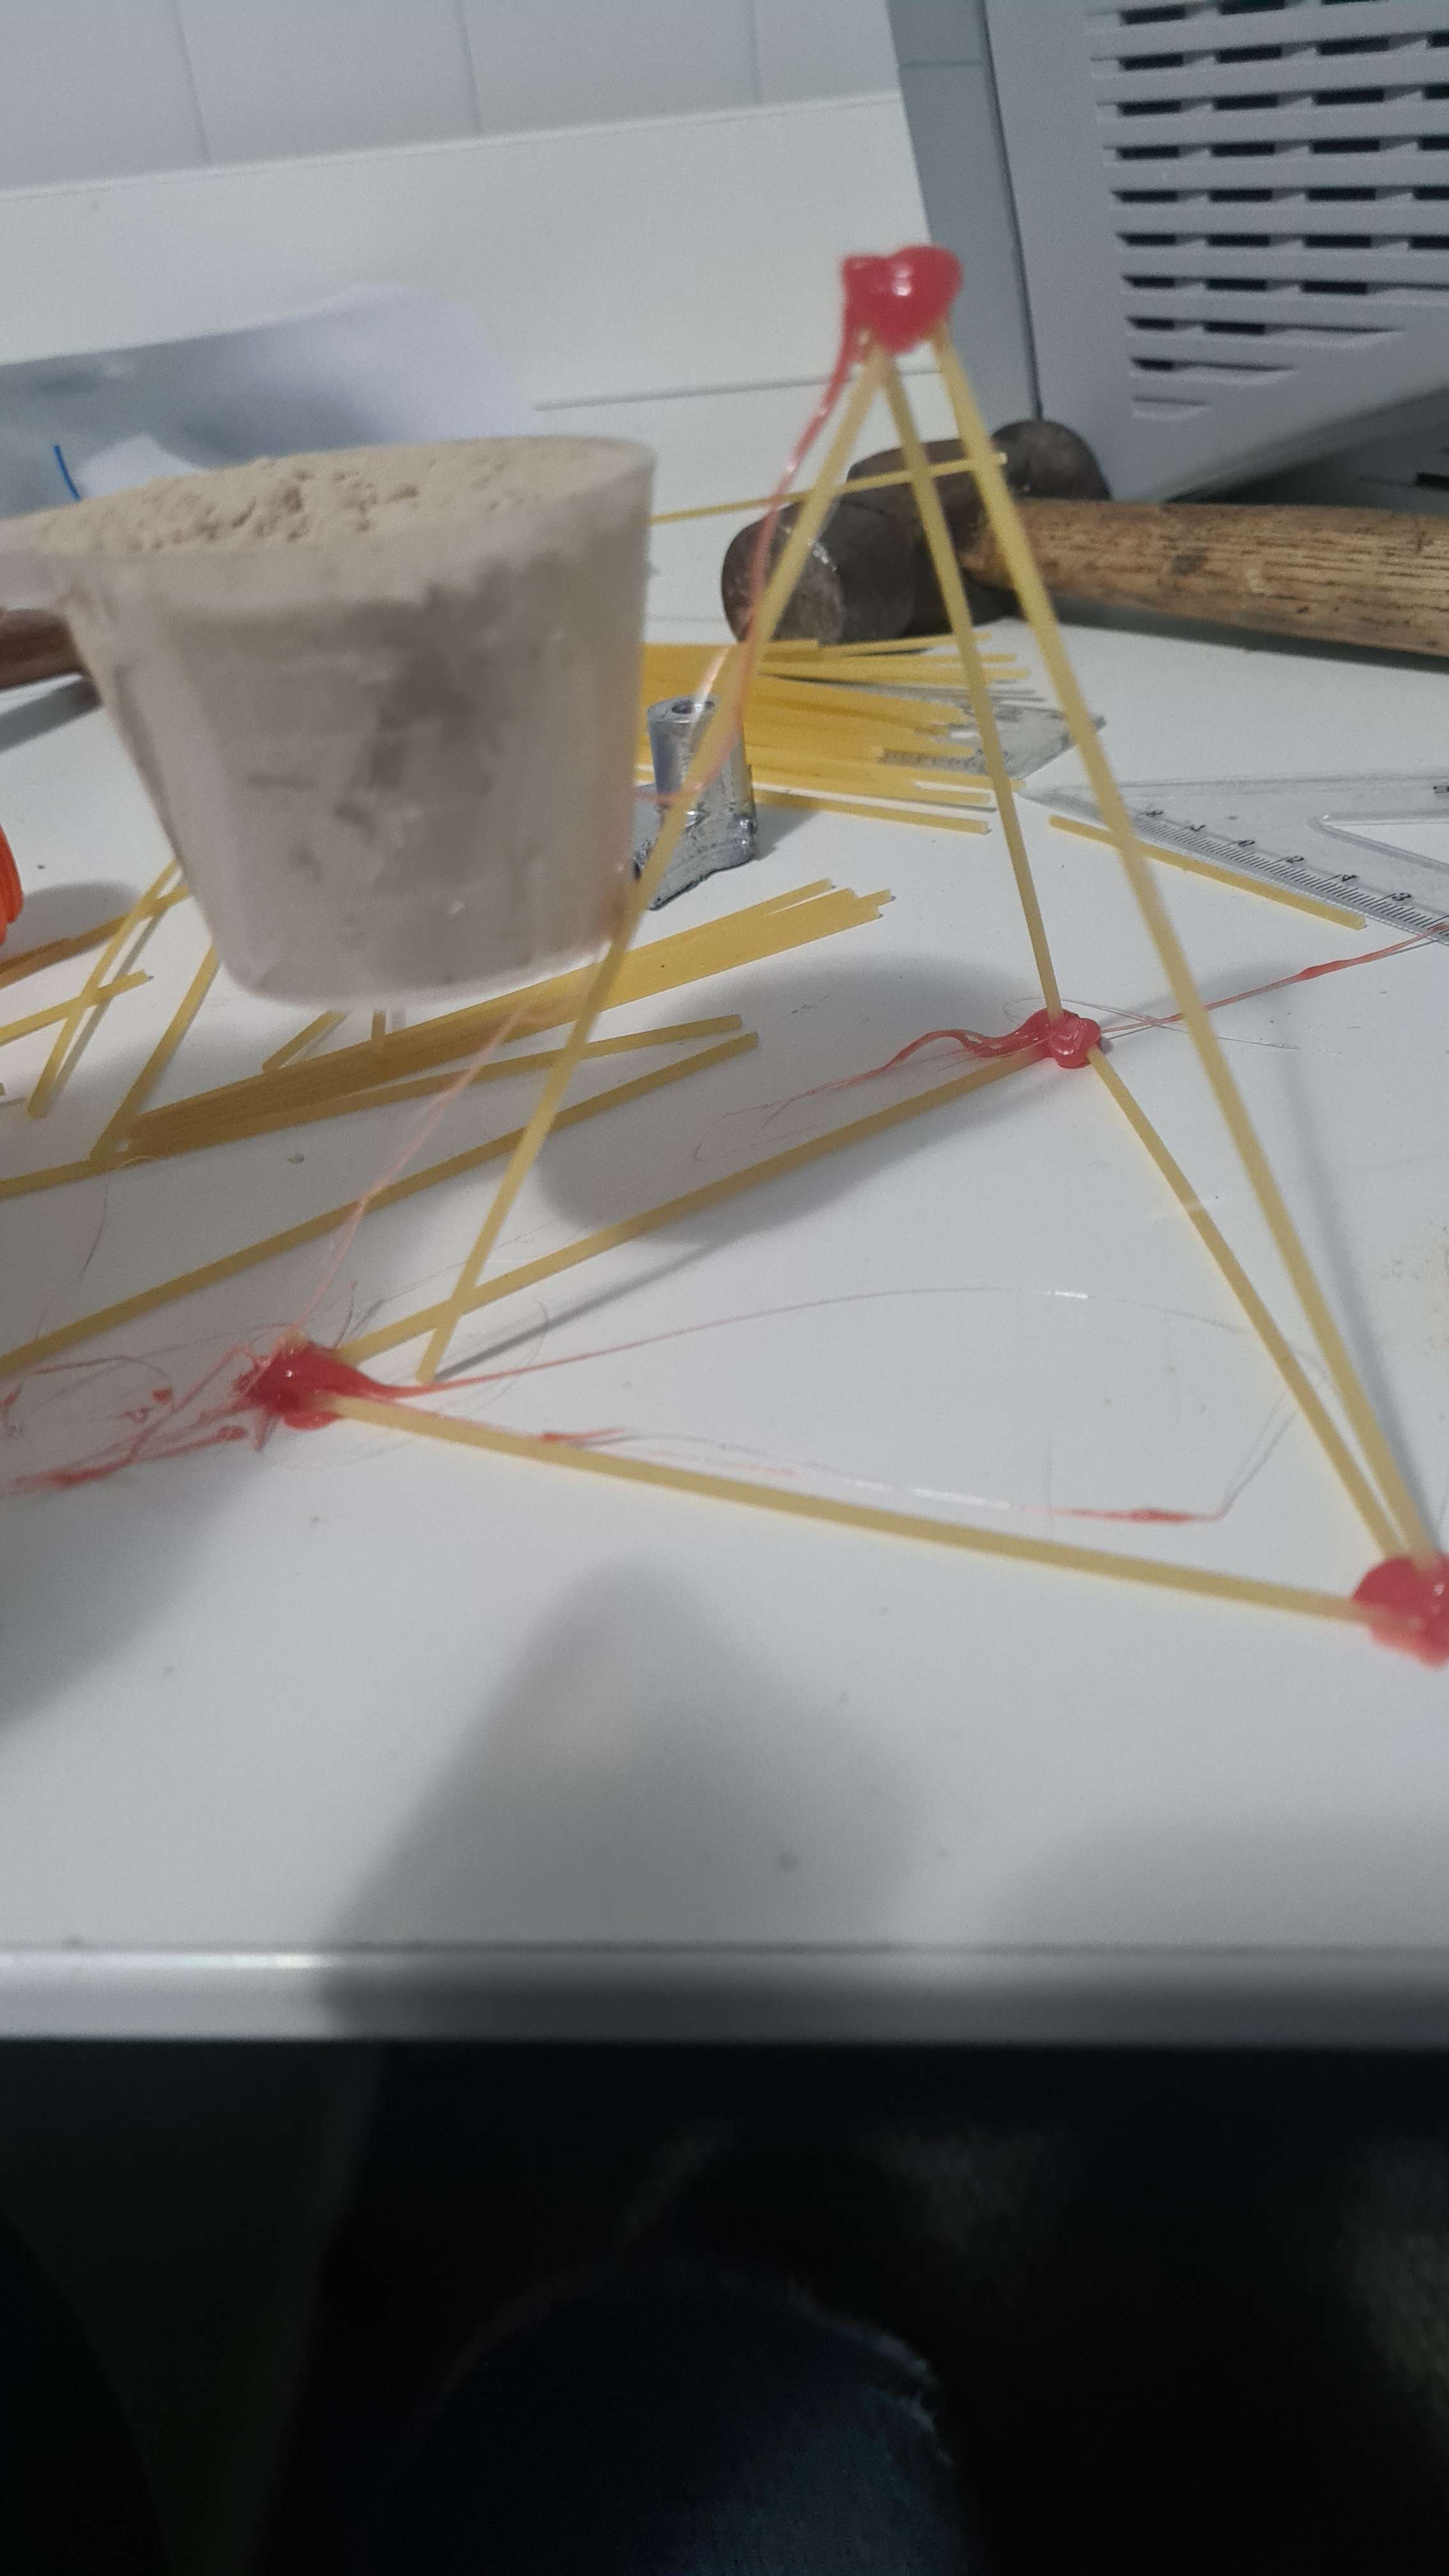
\includegraphics[width=\subimgw]{tetrehedra-b}
		\caption{Buckle force direction of tetrehedra}

		\label{fig:tetrehedra:untranslated}
	\end{subfigure}

	\caption{Tetrehedra}
	\label{fig:tetrehedra}
\end{figure}

Rektangulær trekant har de samme styrkene som en likebeint trekant hvor den korteste kateten tåler mest siden den fordeler kraften på de lengere katetene, men det dumme med rektangulær pyramide er at den kan oppleve planforskyving.

\begin{figure}[H]
	\begin{subfigure}{.5\textwidth}
		\centering
		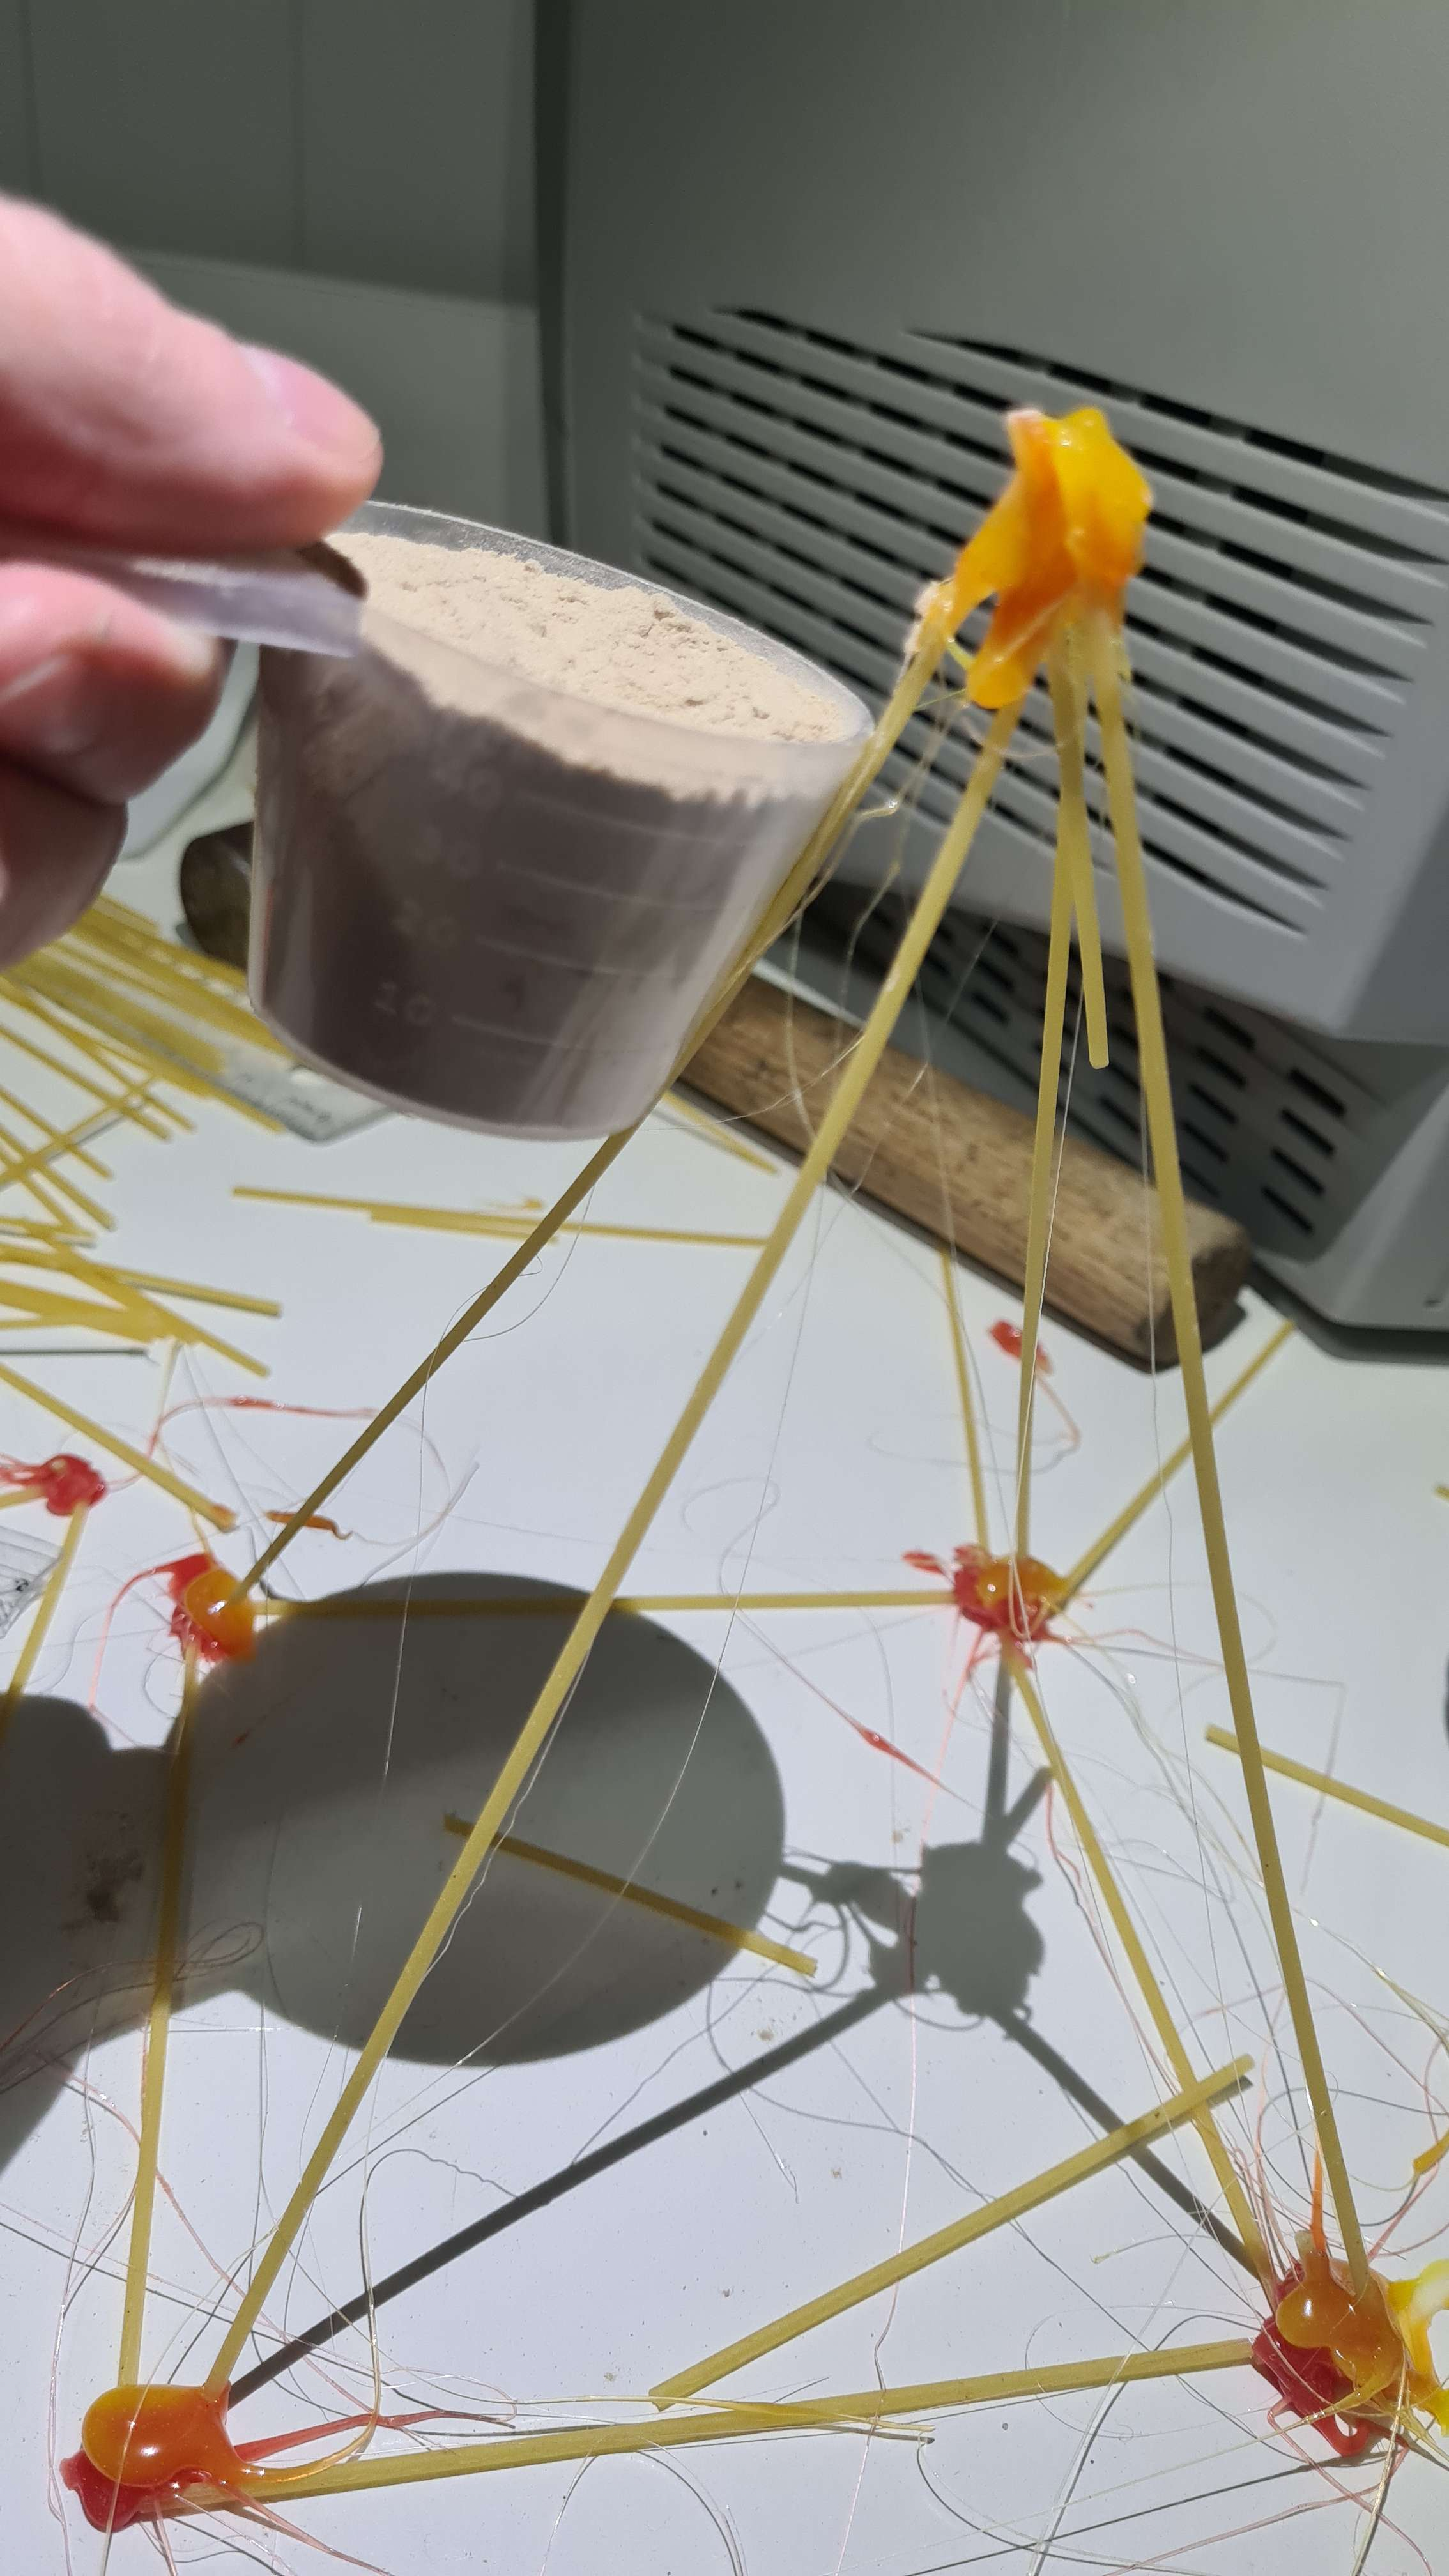
\includegraphics[width=\subimgw]{pyramid-a}

		\caption{Compression bucle of quad-pyramid}
		\label{fig:pyramid:a}
	\end{subfigure}%
	\begin{subfigure}{.5\textwidth}
		\centering
		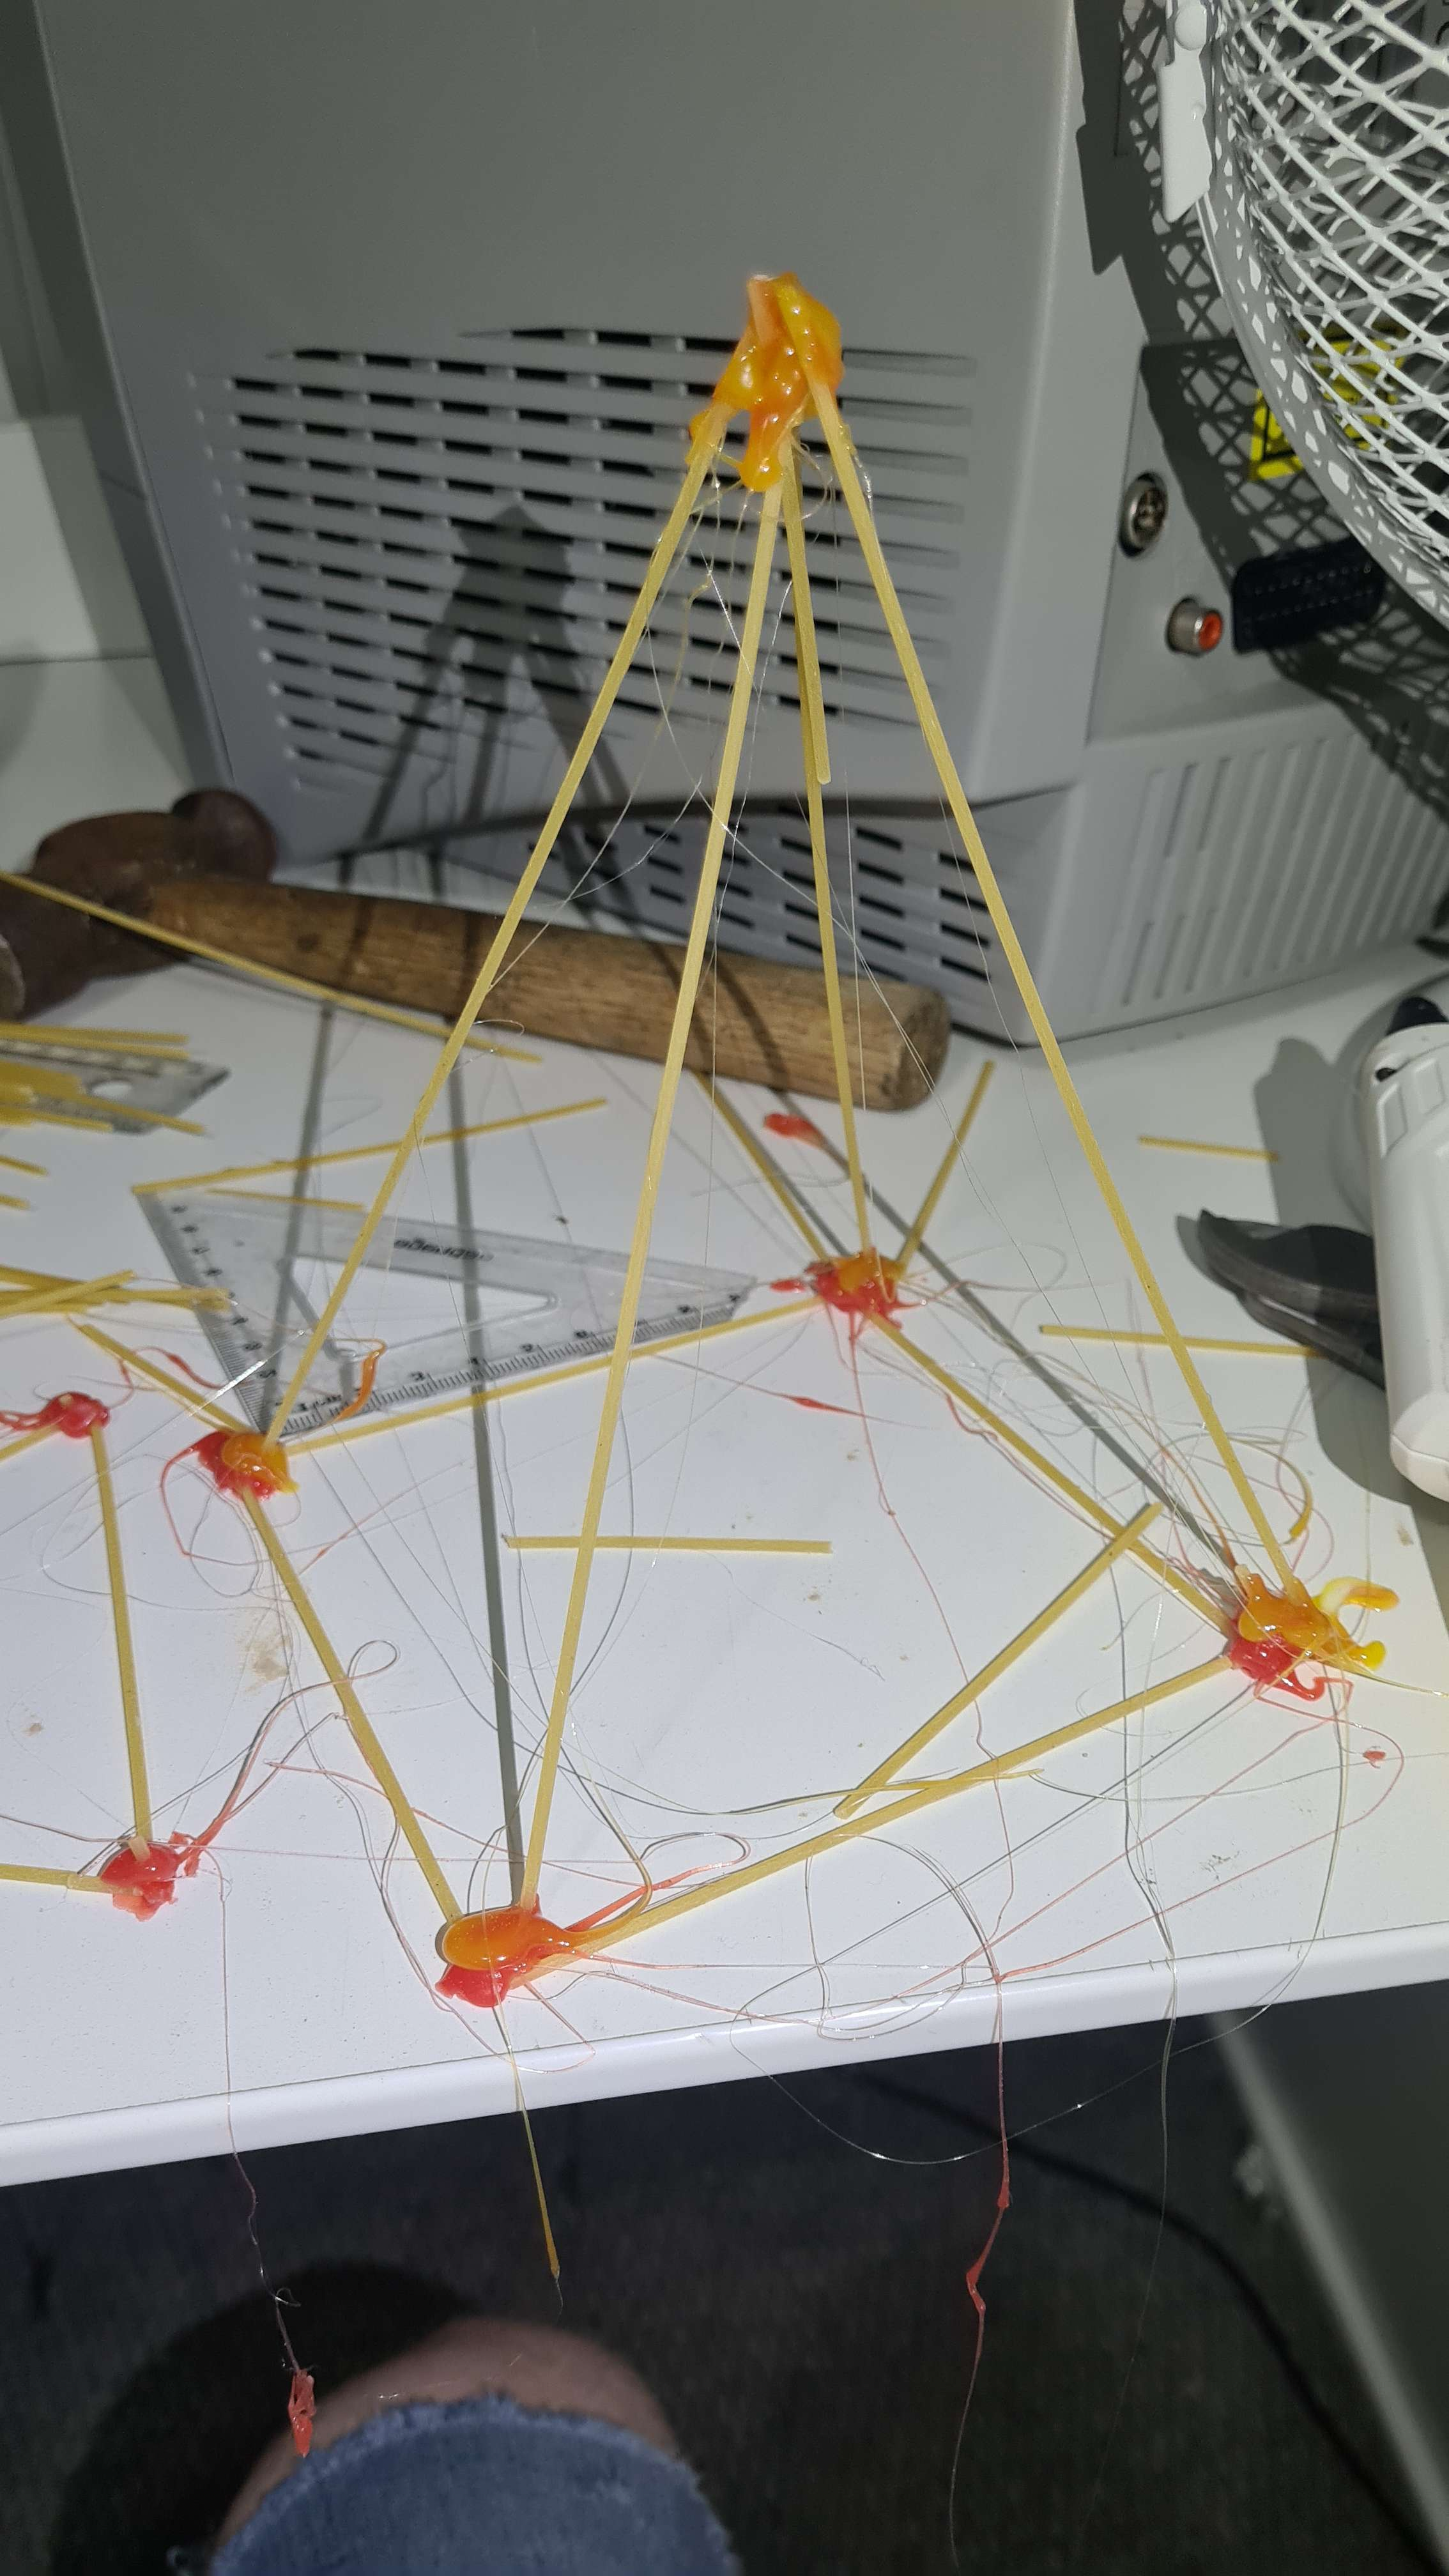
\includegraphics[width=\subimgw]{pyramid-untranslated}

		\caption{Buckle force direction of tetrehedra}
		\label{fig:pyramid:untranslated}
	\end{subfigure}

	\caption{Tetrehedra}
	\label{fig:pyramid}
\end{figure}

En kube er den svakeste formen siden den vil oppleve plan forskyving og knekke enkelt Figure \ref{fig:cube}

\begin{figure}[H]
	\begin{subfigure}{.5\textwidth}
		\centering
		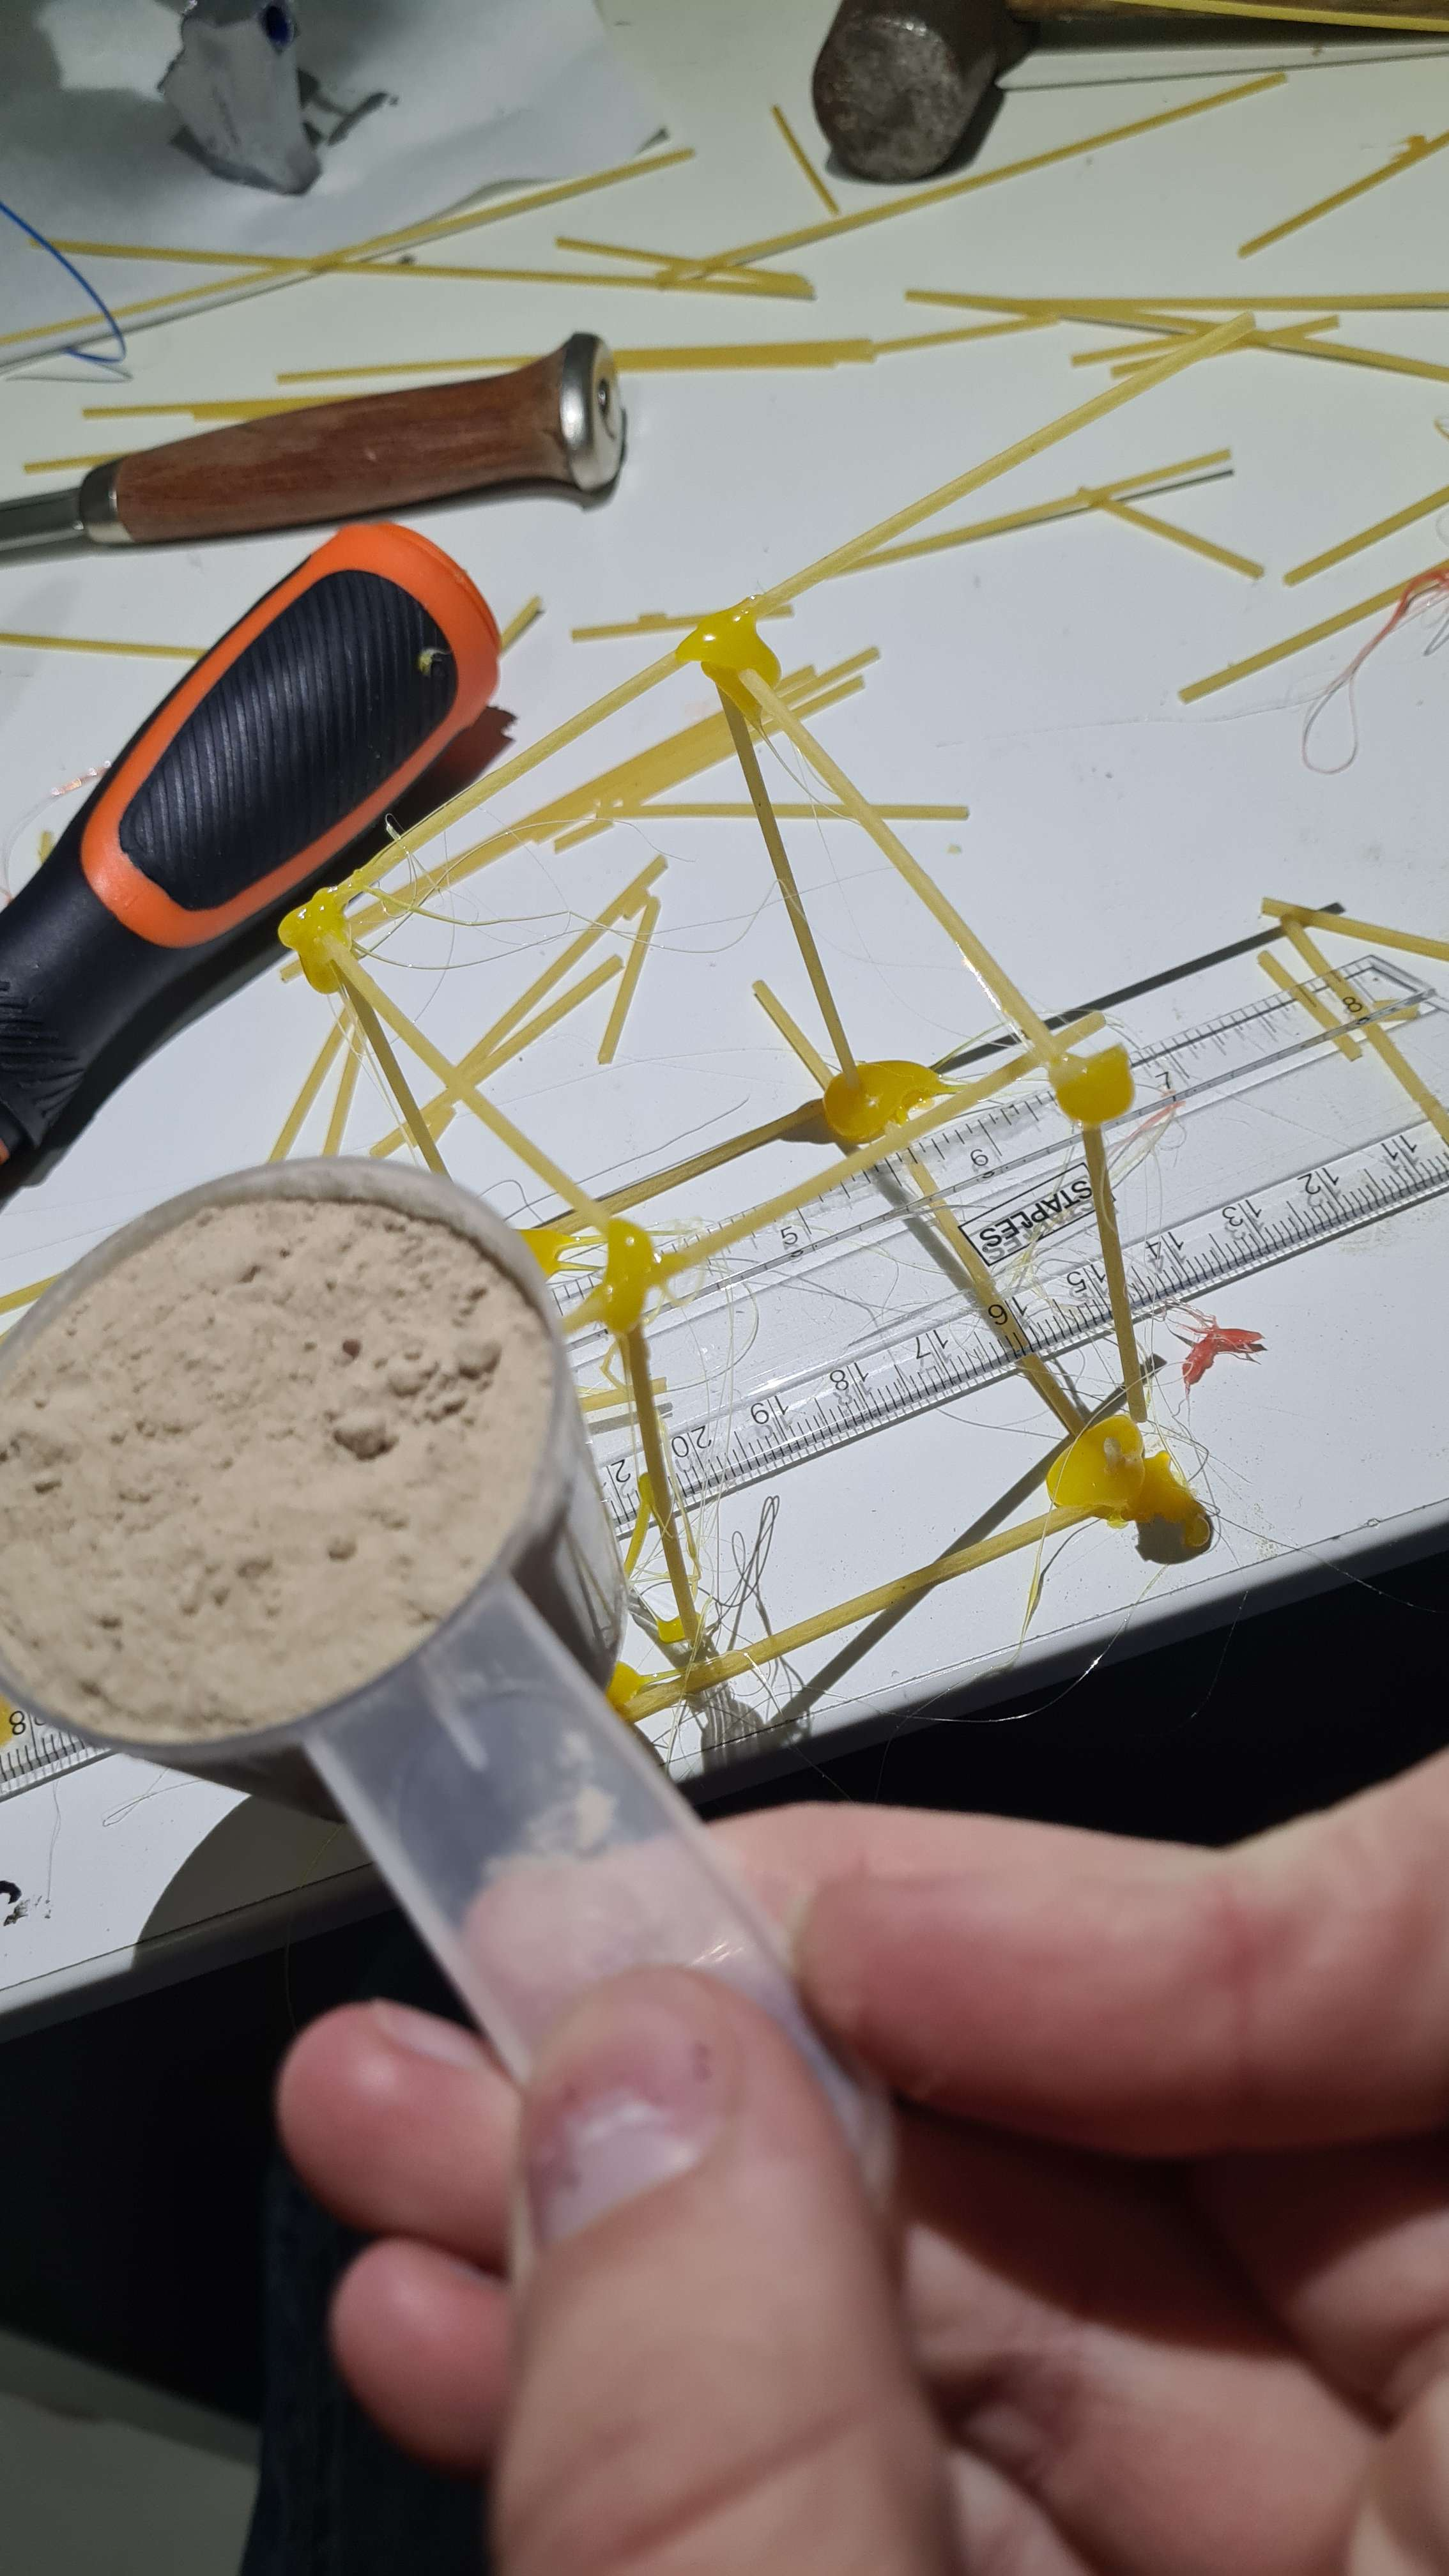
\includegraphics[width=\subimgw]{cube-a}

		\caption{Cube}
		\label{fig:cube:a}
	\end{subfigure}%
	\begin{subfigure}{.5\textwidth}
		\centering
		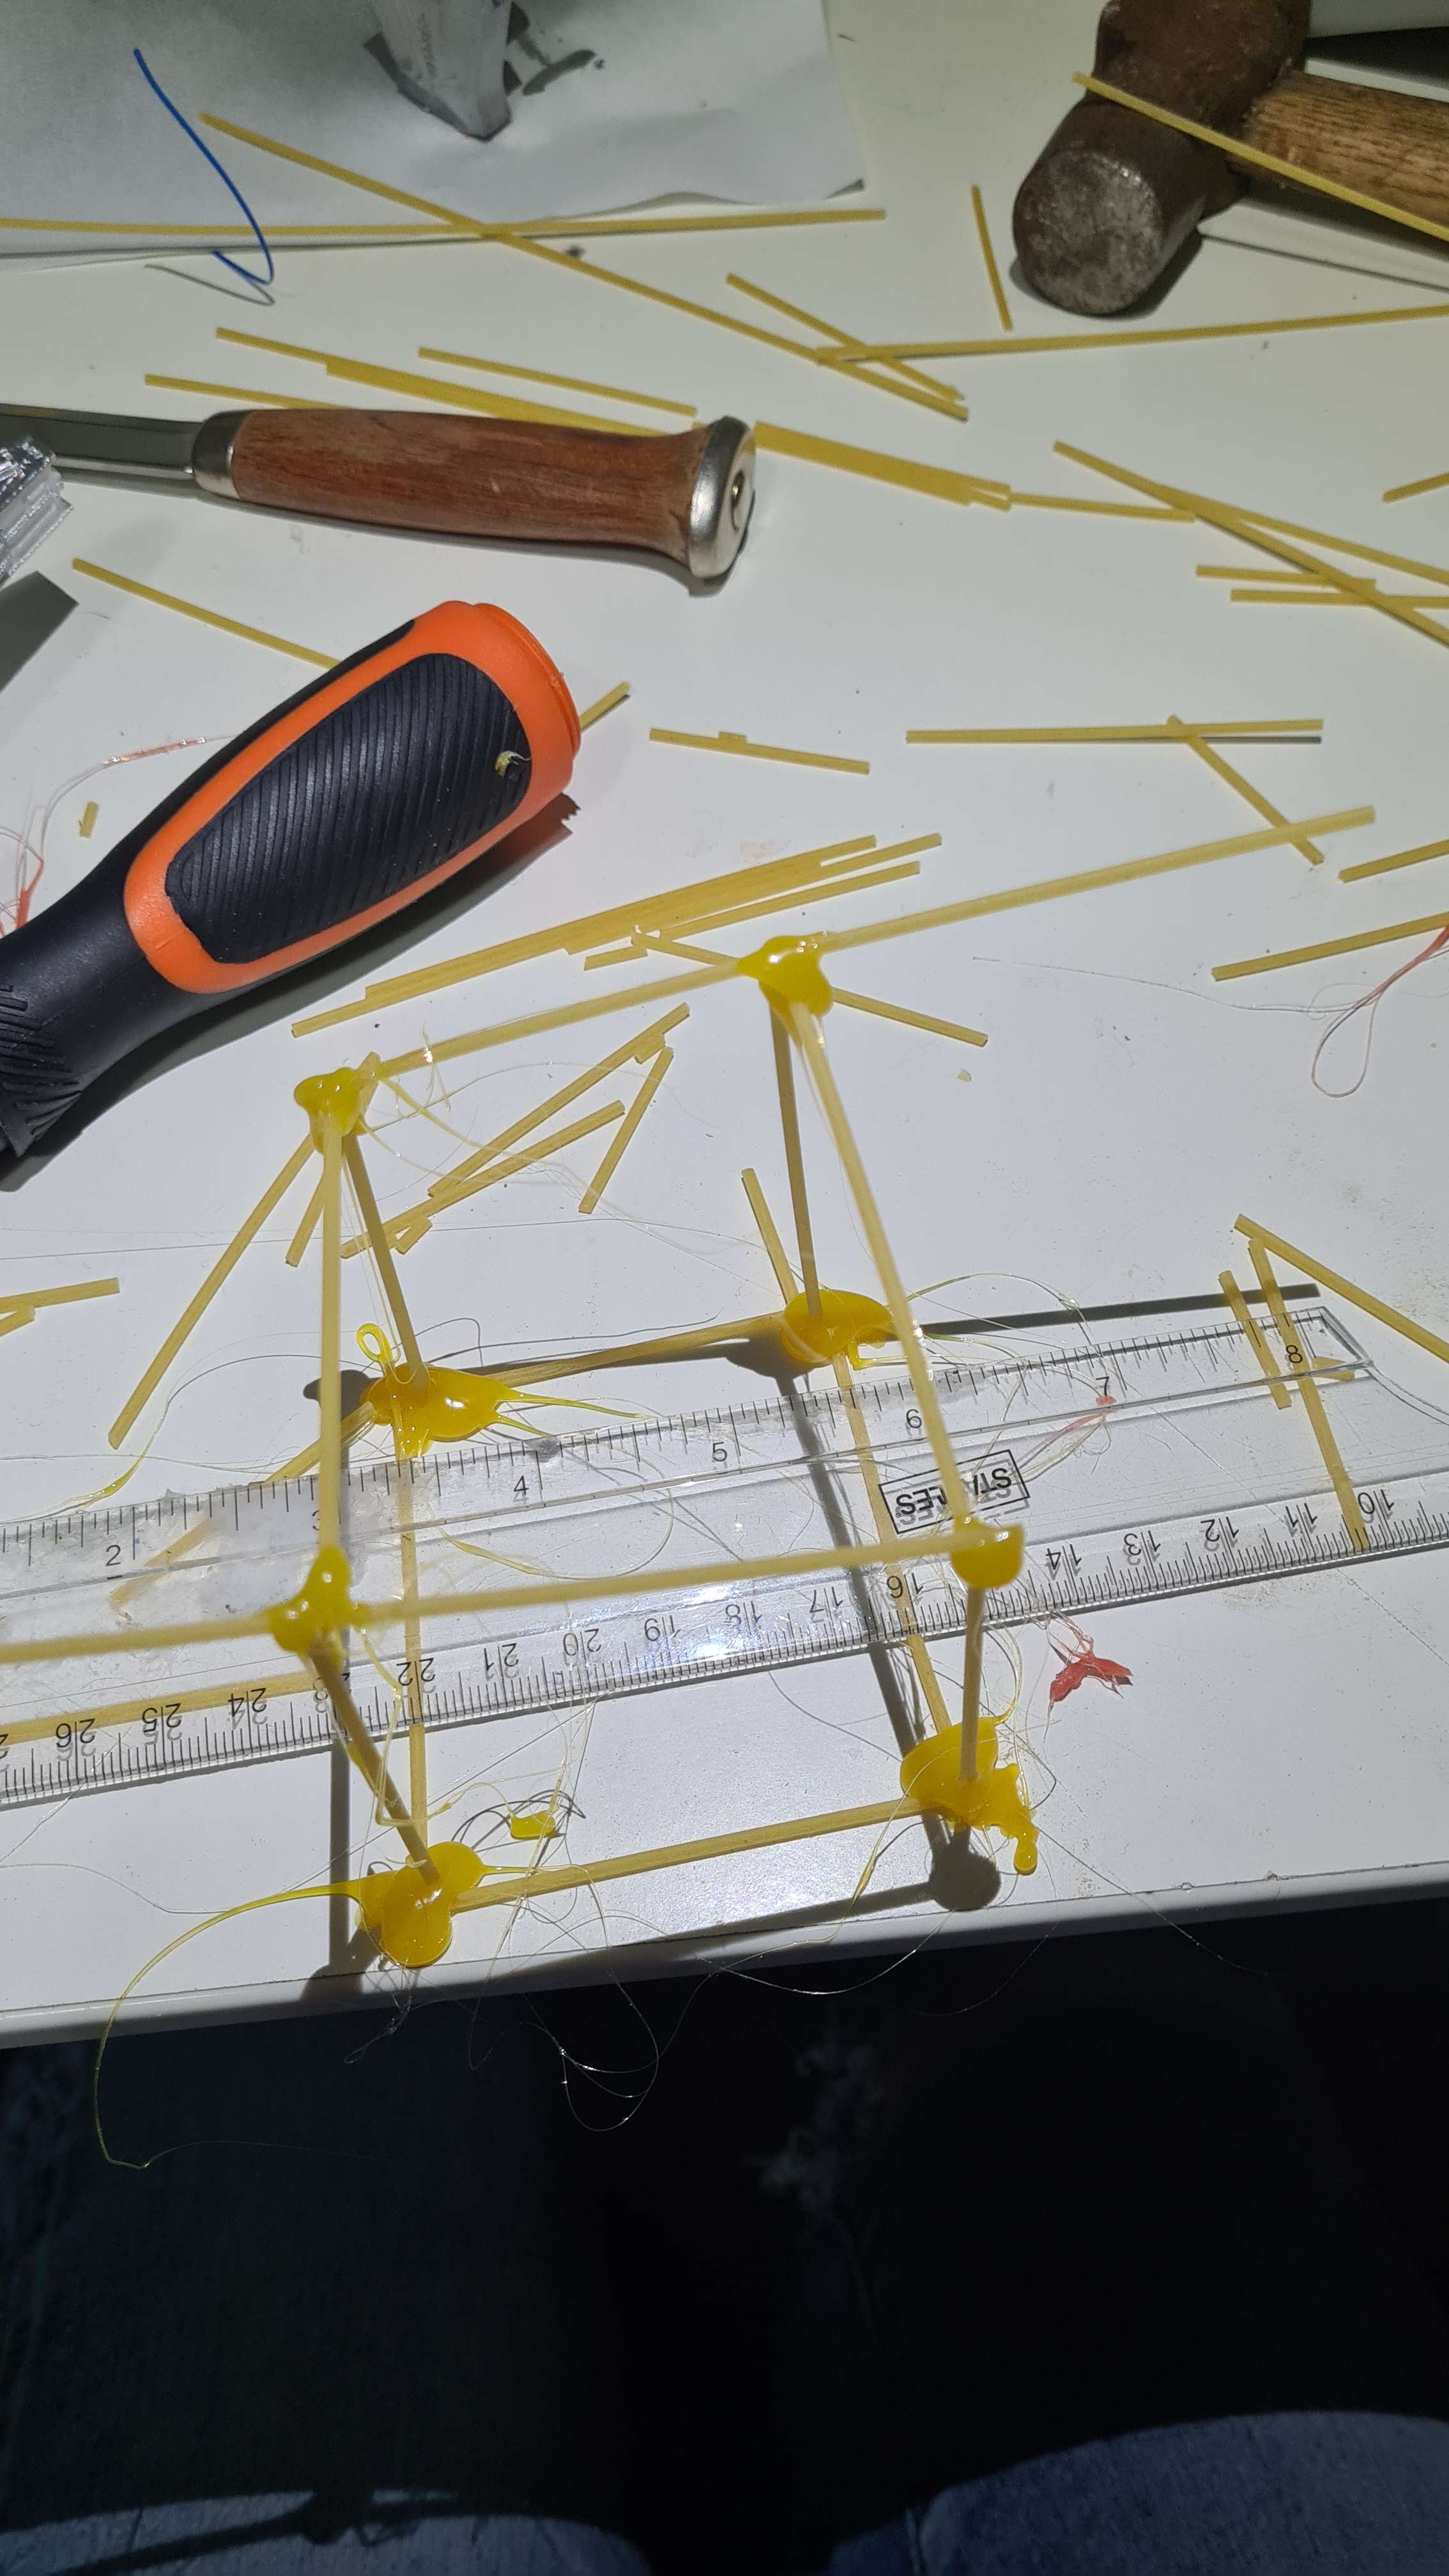
\includegraphics[width=\subimgw]{cube-untranslated}

		\caption{Undemonstartive cube}
		\label{fig:cube:untranslated}
	\end{subfigure}

	\caption{Cube}
	\label{fig:cube}
\end{figure}

\section{Oppgave 2}

% Oppgave 2: Forholds-ligningen og bru-modellens dimensjoner

% I forholds-likningen nedenfor er størrelsene 𝐵, 𝐿 og 𝐻 bruens virkelige bredde, lengde og fri høyde. I denne oppgaven setter vi 𝐵=8,0 meter og 𝐻=4,5 meter. Størrelsene 𝑏, 𝑙 og ℎ er modellbrua sin bredde, lengde og fri høyde. Størrelsen 𝑋 er målestokken. Altså: én cm på modellbrua er 𝑿 cm på den virkelige brua. 𝑏𝐵=𝑙𝐿=ℎ𝐻=1𝑋

% 2A: Velg en passende verdi for 𝑙, 𝑏 eller ℎ, og regn ut målestokken 𝑋 til modellbrua. Bruk målestokken til å regne ut de ukjente verdiene nedenfor. I besvarelsen skal dere kort vise hvordan dere regnet ut alle tallene. Dere kan for eksempel ved å vise svarene og kodene fra Excel eller Python.

% Bredde: 𝑏 cm Lengde: 𝑙 cm eksklusiv landkar.

% Bredde kjørebane: 𝑏𝐾 cm Gang- og sykkelsti: 𝑏𝐺𝑆 cm på hver side.

% Fri høyde: ℎ cm.

% 2B: Vi har flere forskjellige modell-materialer tilgjengelig. Regn ut modell-materialenes virkelige størrelse og modellbrua sin størrelse i henhold til målestokken dere har valgt.

% I besvarelsen skal dere fylle ut tallene som mangler i tabellen nedenfor. Dere må vise hvordan dere regnet ut svarene. Dere kan for eksempel løse oppgaven ved å bruke Excel eller Python, og vise kodene.

I denne oppgaven skulle man regne ut en målestokk for gruppens modellbru. Dette gjør mann med å bruke bruen virkelige størrelse og dele det på gruppens utvalgte målestokk

\subsection{a}

Vi bruker lengden til bruen til å regne ut målestokken. Lengen på modelbruen er $80\mathrm {cm} = 0.80\mathrm m$, den ekte bruen er $28\mathrm m$ (klasse A). Da får vi $\frac {25} {.8} = 31.25$.

\subsection{b}

\section{Oppgave 3}

\begin{figure}[H]
	\centering
	\includegraphics[width=.8\linewidth]{frame00000}

	\caption {OpenSCAD dump of bride including a legend of the different measurements.}
	\label{fig:bridge}
\end{figure}

I oppgave 3 skulle man bruke målestokken man har regnet ut tidligere for å lage en arbeidstegning. Dette skulle egentlig gjøres på ark som ble gjort, men når dette ble gjort var ikke tegningen nøyaktig og den ble heller programer inn i open SCAD for å få den mest mulig nøyaktig.

\section{Oppgave 4}

\textbf {Lofoten}

Fisk: Lofoten er kjent rundt om i verden for sin fisker kultur. Derfor måtte vi intigrere deres kultur in i vårt bru design. Så det er 3d printed flere båter og fisker som kan festes på for å symbolisere dette.

Pride: Lofoten er blant de kommunene med høyest rate av mennesker som aksepterer homofile. Dette er også blant de kommunene som var først til å vie homofile med grunnlag på at dette var den kommunen med den første homofile presten og i dag er opp mot halvparten av prestene i kommunen homofil. dette er grunnen til at vår bru har et pride flag festet på seg

Miljø: det å bygge en bru er en prosess som krever mye energi og ressurser som er veldig skadelig for miljøet. Ifølge Architecture 2030 så står Bygg og konstruksjons industrien for 40\% av årlige utslipp dette er grunnen til at vår bru er bygget med sol celle panel slik at bruen etter mange vil bli karbon nøytral og i tillegg hjelpe lokal miljøet

\section{Oppgave 5}

Som blir å synes i besverelse i oppgave 7 har vi bestemt oss for å modelere bruen vår som en $\cosh$ funksjon. Gjennom dette og litt geometrisk resonemang har det ledet oss til å lage et simulasjons generasjons program som ligger Appendix \ref{sec:jhu-gen}. Denne koden genererer en JHU save file som så lastes inn og man utfører simulasjonen. Dette resulterer så i Figur \ref{fig:jhu} der du kan se resultatet av simuleringen.

\begin{figure}[H]
	\centering
	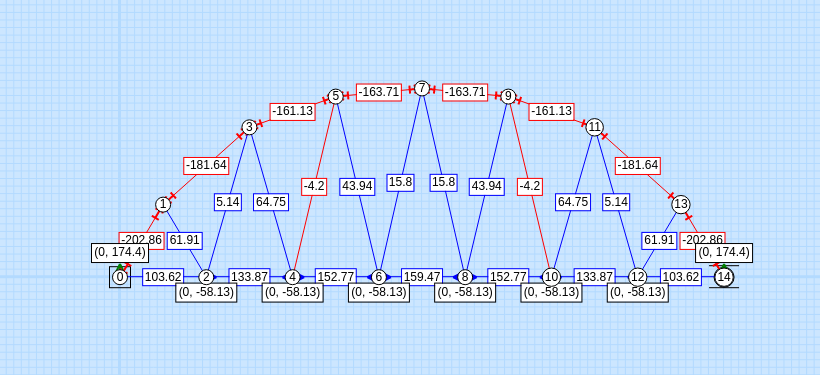
\includegraphics [width=.8\linewidth]{jhu}
	\caption{Jhu simulation of bridge from generation code}
	\label{fig:jhu}
\end{figure}

Vi har bestemt oss for å ikke inkludere "member list" i dette dokumentet siden det kan trivielt uthentes av generator programmet; kjør generator programmet og undersøk outputet.

\section{Oppgave 6}

Koden for utførelse av oppgave 6 er lokalisert i Appendix \ref{sec:jhu-gen} sammen med JHU-gen koden. Kjører du programmet så ser du at den printer all informasjon som skal til. Dette er \lstinline{total_force_irl} og \lstinline{pascal} som svar på 6a, \lstinline{roind(distribution,2)} er svar på 6b, \lstinline{total_force_model} og \lstinline{round(total_force_model/g,2)} er svar på 6c.

\subsection*{D}

TODO

\section{Oppgave 7}

\subsection {Hvorfor $\cosh$}

Vi har bestemt oss for å modelere bruen som en $\cosh$ kurve gjennom at den er grunnlaget for en catenery curve: kurven som minimaliserer potensiel energi av en funksjon \cite{wiki:catenery}. Gjennom at den minimaliserer potensiel energi så er det også den sterkeste mulige kurve med get en gitt lengde på archen.

\subsection {Feiler under bygging}

Under første iterasjon av broen så brukte vi spheriske knutepunkter. Dette var negativt for flere grunner.
\begin{enumerate}
	\item Det kaster bort plastik; vi trenger ikke det extra toleranse for rotasjonelle krefter.
	\item De var vanskelig å printe; vi trengte extreme mengder med supports og i noen tilfeller supports vi ikke kunne fjerne.
\end{enumerate}

\subsection {Features av slutt bruen}

\subsubsection {Percentage extending baserods}

Gjennom designet så vi at vi trenger å feste grunnstavene sammen. Dette var et problem vi bestemte oss for å løse med å legge til en utvited nederst rod. Dette kan synes i Appendix \ref{sec:openscad}:\ref{line:brescale}. Vi endte opp med å velge en extention faktor av \lstinline{BASE_RESIZE = 6}.

\subsubsection {Stabelizing backplate}

Gjennom testing så vi at extention pinnene som knutepunktet består av kunne brekke av. Dette var noe vi så kompanserte med av å lage en poligonal backplate. Denne backplaten sin struktur er refrencet i Appendix \ref{sec:openscad}:\ref{line:backplate}. Kodestilen brukt er variabler i static single-assignment form \cite{wiki:ssaf}.

\subsubsection {Internailzed standoff}

Når vi bygget bruen måtte vi sande ned medlemmene til å kunne feste dem sammen. Dette var et problem gjennom at vi ikke hadde rett presisjon. For å fixe dette la vi til internaliserte standoffs som lot oss sette staver inn uten å måtte pusse ned medlemmene.

\subsubsection {Node indexing}

Vi så etter første print batch at vi hadde ingen måte å identifisere knutknutepunktene. Til å fixe dette endte vi opp med å lagge til en identifiserende index på hvert punkt. Dette lot oss også si nøyaktig lengde på hvert av medlemmene til og fra knutepunkter.

\subsubsection {Cross section margin connections}

Vi så at de tversående medlemmene hadde hengt dorlig i kværandre gjennom at det var lite matriale deligert til dem i hvert knutepunkt. Til å fixe dette la vi til en margin som vi kunne.

\subsubsection {Lamination direction}

Vi hadde bestemt oss for å printe på sånn et vis at vi fikk infille i den rette rettningen.

\chapter{Appendix}

\section{Refrence to OpenSCAD code}
\label{sec:openscad}

\lstinputlisting[escapechar=~]{../bridge.scad}

\section{Recrence to Python JHU-generation code}
\label{sec:jhu-gen}

\lstinputlisting[language=Python]{../jhu-gen.py}

\addcontentsline{toc}{section}{List of figures}
\listoffigures

% \bibliography{report}

\end{document}

